\documentclass[a4paper,10pt]{scrartcl}
\usepackage[ngerman]{babel}
\usepackage[T1]{fontenc}
\usepackage[utf8]{inputenc}
\usepackage{graphicx}
\usepackage{underscore}
\usepackage{listings}
\usepackage{color}

\definecolor{dkgreen}{rgb}{0,0.6,0}
\definecolor{gray}{rgb}{0.5,0.5,0.5}
\definecolor{mauve}{rgb}{0.58,0,0.82}

\lstset{frame=tb,
	language=Java,
	aboveskip=3mm,
	belowskip=3mm,
	showstringspaces=false,
	columns=flexible,
	basicstyle={\small\ttfamily},
	numbers=none,
	numberstyle=\tiny\color{gray},
	keywordstyle=\color{blue},
	commentstyle=\color{dkgreen},
	stringstyle=\color{mauve},
	breaklines=true,
	breakatwhitespace=true,
	tabsize=3
}

\title{Software Engineering 3}
\author{Benjamin Altmiks}
\date{8. Oktober 2018 - \today}

\begin{document}
\tableofcontents
\maketitle

\section{Einleitung}
\subsection{Rückblick}
        \textbf{Zeit:}      Bei Zeit wird Start und Enddatum/Stunde verwendet. Es ist nicht relevant wie viele Personen an dem Projkt beteiligt waren.
\newline\textbf{Kosten:}    Äquivalent zur Zeit, da die Areitszeit bezahlt werden muss. 
                                Hier ist es relevant wie viele Personen an diese Projekt gearbeitet haben da ealle bezahlt werden müssen.
\newline\textbf{Qualität}:   Unterscheidung zwischen Produktqualität und Prozessqualität.
\begin{itemize}
    \item Produktqualität: Der ganze Prozess, das beeinhaltet Brauchbarkeit und Wartbarkeit 
    \item Prozessqualität: Das Endprodukt, das Ergebniss, das heißt die Software selber
\end{itemize}
\section{Architektur}
\subsection{Allgemein}
\begin{quote}   "Architektur ist schwer greifbar" \newline -Vogel   \end{quote}
Architktur ist ein sich selbst durch die Evolution entwicklender Prozess. Sie ist ein universeller Bestandteil/Grundriss von Software
\begin{quote}    "... werden Entwickler, wenn auch oft unbemerkt, in ihrer täglichen Arbeit mit Architektur konfrontiert, weil diese impliziet immer ein Aspekt von
Software ist und sich nicht eliminieren, allenfalls ignorieren lässt." \newline -Vogel    \end{quote}
\textbf{Softwarearchitektur ist eine strukturierte oder hierarchische Anordnung der Systemkomponenten sowie Beschreibung ihrer Beziehungen. Diese nennt man häufig Architekturmuster}
\newpage
\subsection{Architekturmuster}
Architekturmuster versuchen eine grundlegede Organisation und Interaktion zwischen Komponenten einer Anwendung her zu stellen. Man unterscheidet allgemein Strukturierende Architekturmuster, Muster für Interaktive Systeme und Muster für verteilte Sytsteme

\subsubsection{Strukturierende Architekturmuster}
\textbf{Pipes und Filter}
\begin{itemize}
    \item Beschreibt die Struktur für Systeme, die Datenströme verarbeiten.
    \item Filter = Verarbeitungsschritt mit Dateneingabe und Datenausgabe
    \item Pipes = Verbindung zwischen einzelner Komponenten \newline
    $\Rightarrow$ Verschiedene, unabhängige Komponenten für flexible, unterschiedliche Aufgaben
\end{itemize}
\textbf{Schichten}
\begin{itemize}
    \item Aufteilung auf Schichten für große/komplexe Systeme 
    \item Ziel ist eine Abhängigkeitslösung der Komponenten zu erreichen\newline
    $\Rightarrow$ Austauschbarkeit und Integration neuer Systeme einfacher möglich
    \item Ein Besipiel ist das OSI-Schichtenmodell bei Netzwerkprotokollen
\end{itemize}
\subsubsection{Architekturmuster für interaktive Systeme}
\textbf{Model-View-Controller}\newline
Einteilung in drei Komponenten:
\begin{enumerate}
    \item Datenmodell (model): Enthält die Daten die dargestellt werden. Ist unabhängig von anderen
    \item Präsentation (view): Darstellung der Daten des Modells mit Benutzerinteraktion
    \item Programmsteuerung (controller): Benutzerinteraktionen verwaltet Präsentation und Datenmodell
\end{enumerate}
$\Rightarrow$ Reduzierung von Abhängigkeiten, Benutzerschnittstellenorientiert  \newline
\begin{figure}[h]
	\centering
	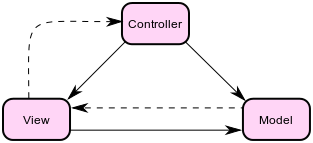
\includegraphics[width = 4.5cm]{ModelViewControllerDiagram2}
\end{figure}
\newpage
\subsubsection{Architekturmuster für verteilte Systeme}
\textbf{Vermittler-Prinzip}

\begin{itemize}
    \item Verteiltes System mit (unabhängigen) Komponenten, die zusammenarbeiten 
    \item Vermittler steuert Objekte, Objekte nicht untereinander\newline
    $\Rightarrow$ Einfache Kombination von Diensten und Objekten in einem System
\end{itemize}
\textbf{Client-Server}
\begin{itemize}
    \item Verteilte Benutzer mit zentraler Anwendung 
    \item Verschiedene Funktionalitäten durch Verteilung auf Netzwerkkomponenten\newline
    $\Rightarrow$ Beispiele sind das WWW oder E-Mail 
\end{itemize}
\subsubsection{Zusammenfassung}
\begin{itemize}
    \item Architektur bringt keinen direkten Mehrwert für die Software mit sich
    \item Funktionale Zusätzliche Fähigkeiten und Flexibilität der Software besser\newline
    $\Rightarrow$ Zukunftssichere Software (Kostengünstiger, Zuverlässiger)
    \item Gute Architektur ist eine notwendige, aber keine hinreichende Voraussetzung für gute Qualität
\end{itemize}
\subsection{Micro- und Marko Architektur}
Allgemein werden beide benötigt um die Effizienz des Entwicklungsprozesses zu verbessern.
\subsubsection{Microarchitecture TODO}
Micro Architektur betrachtet die Software Entwicklung „von Unten”, legt also den Fokus auf auf
kleine Einflüsse.
\begin{itemize}
    \item \textbf{FUTUR} Eine Future stellt der Rückgabewert einer Berechnung dar, der zur Zeit noch nicht verfügbar ist.
    \item \textbf{CALLBACK}
    \item \textbf{LISTENABLEFUTURE}  Kombination aus Future und Callbacks
    \item \textbf{PROMISES}
\end{itemize}

\subsubsection{Event}
Ein Ereignis (englisch Event) dient in der Softwaretechnik – bei Entwicklung nach dem ereignisorientieren Programmierparadigma – zur Steuerung des Programmflusses. Das Programm wird nicht linear durchlaufen, sondern es werden spezielle Ereignisbehandlungsroutinen (engl. listener, observer, event handler) immer dann ausgeführt, wenn ein bestimmtes Ereignis auftritt. Ereignisorientierte Programmierung gehört zu den parallelen Programmiertechniken, hat also deren Vor- und Nachteile.
\begin{itemize}
    \item + Sehr einfach neue Systeme umzusetzten 
    \item + Jedes abhängige System kann seine Sicht auf die Daten vorhalten. Vermeidung von „Resource contention”
    \item - Es ist nicht einfach, festzustellen, welche Systeme voneinander abhängen
    \item - Konsistenz: Die Datenmodelle sind nur noch „eventually consistent”
\end{itemize}
$\Rightarrow$ Events werden generiert wenn eine Veränderung am Datenmodell vorgenommen wurde. 
\subsection{Architektur Dokumentieren}
\subsubsection{Wie viel Architektur Dokumentation ist sinnvoll?}
Man muss berücksichtigen:
\begin{itemize}
    \item Nutzen des Dokuments für Entwickler, neue Mitglieder des Teams, etc.
    \item Den Aufwand, das Dokument zu pflegen
\end{itemize}
$\Rightarrow$ Wägen Sie für jedes Projekt ab, welche Dokumentation sinnvoll ist.
\subsubsection{Feste Gliederung}
\textbf{Vorteile}: Einheitliche Gliederung für alle Autoren mit einfacher Vollständigkeitssicherung. Neue Mitglieder und Reviews einfacher. \\
\textbf{Nachteile}: Form über Inhalt, Vollständigkeitsmengel\\
\subsubsection{arc42}
\begin{itemize}
    \item Aufgabenstellung: Architektur Dokumentation über Schach-Engine
    $\Rightarrow$ Feauters sind Schachregeln, Taktiken, User vs AI oder AI vs AI, Integration
    \item Qualitätsziele
    $\Rightarrow$ Analysierbarkeit, Änderbarkeit, Interoperabilität, Attraktivität
    \item Stakeholder
    $\Rightarrow$
\end{itemize}

\section{Testen und Verifizieren}
\subsection{Allgemein}
\subsubsection{Fehlerarten}
Grundsätzlich müssen die verschiedenen Fehlern untereinander abgegrenzt werden. 
\begin{itemize}
	\item Fehlbedienung: "Die bedienende Person verwendet das Programm nicht wie vorgesehen. Ein Person macht einen Fehler." 
	\footnote{Prof. Dr. Phillip Heidegger: "'Software-Engineering 3", S. 213}
	\item Defekt: "Fehlerhafte Stelle des Programms, die ein Fehlverhalten auslösen kann. Die Anwendung enthält einen Fehler." \footnote{Prof. Dr. Phillip Heidegger: "'Software-Engineering 3", S. 213}
	\item Fehler: "Fehlverhalten eines Programms gegenüber der Spezifikation, dass während seiner Ausführung auftritt. Die Anwendung zeigt einen Fehler."
	\footnote{Prof. Dr. Phillip Heidegger: "'Software-Engineering 3", S. 213}
	\item Infektion: 
\end{itemize}

\subsubsection{Testtechniken}
Es wird zwischen der statischen und der dynamischen Testtechnik unterschieden. 
\footnote{vgl. dazu https://www.software-testing.academy/software-testing-methoden.html}
\begin{itemize}
	\item Dynamischen Tests: Ausführen des Programms
	\begin{itemize}
		\item Execution-Based-Method
		\item Kontrollierte Ausführung der zu testenden Software mit Erstellung von Testfällen mit konkreter Eingabe und zu erwartenden Ausgabe
		\item BlackBox-Technik, WhiteBox-Technik
	\end{itemize}
    \item Statische Tests: Anschauen des Programmcodes
    \begin{itemize}
    	\item Non-Execution-Based-Method
    	\item Erstellung von Code Reviews oder werkzeuggestützter statischer Analysen
    	\item Nutzung der menschlichen Denk- und Analysefähigkeiten
    \end{itemize}
\end{itemize}
$\Rightarrow$ Das Ziel ist möglichst viele Fehler zu finden und diese zu reparieren.
\newpage
\subsection{Lösung eines Fehlers}
Das Allgemeine Vorgehen zum Lösen eines Fehlers
\begin{enumerate}
    \item Breakpoint setzten und Fehlverhalten immer weiter eingrenzen
    $\Rightarrow$ Oft gibt es viele Infizierte Stellen
    \item Je größer die Software, desto schwerer ist abzuschätzen wo der Fehler ist.
    \item 
    \item 
\end{enumerate}
\newpage
\subsection{Korellation vs Kausalität}
\subsubsection{Korellation}
Zwei oder mehrere Merkmale müssen keine Beziehung zueinander haben. Sie beeinflussen sich gegenseitig nicht, können aber eine Zufällige Beziehung zueinander haben.
\subsubsection{Kausalität}
Eine Ursache-Wirkung Beziehung, betrifft also die Abfolge aufeinander bezogener Ereignisse und Zustände.
\newpage

\subsection{Assert}
    Ein Assert ist Teil eines Programms, welches eine Erwartung ausdrückt. Speicherstellen werden gegen erwartete Werte getestet. Dadurch können Programmfehler zur Laufzeit beim Anwender entdeckt werden. Es wird versucht die erste Infektion im Programm zu finden, um damit die Ursache im Code zu schließen.\\
    Einfaches Beispiel in Java:
    \footnote{vgl. dazu http://www.linkfang.de/wiki/Assertion_(Informatik)}
    \begin{lstlisting}
    int n = readInput(); 
    n = n * n; //Quadrieren 
    assert n >= 0;
    \end{lstlisting}
    Mit dieser Assertion sagt der Programmierer: "' Ich bin mir sicher, dass nach dieser Stelle n größer gleich null ist".\\
    $\Rightarrow$ "'Asserts können dazu beitragen, Infektionen klein zu halten,(...)"
    \footnote{Prof. Dr. Phillip Heidegger: "'Software-Engineering 3", S. 225}
	\\\textbf{Fail-Fast-Einsatz:}\\
	Frühzeitige Erkennung von Fehlern um Schnittstellen abzusichern. (Eingrenzung von Distanz zwischen erster Infektion und Beobachtung)
	\\\textbf{Design by Contact (Entwurf gemäß dem Vertrag):}\\ Definition formaler Verträge zur Verwendung von Schnittstellen. Dieser Vertrag besteht aus Vorbedingungen, Nachbedingungen und Invarianten(Invariant = Vor und nach Befehl Gültig). Asserts können Verträge für Methoden darstellen.
	\\\textbf{Java Modelling Language (JML):}\\
	Eine Alternative Möglichkeit zu Asserts zur Angabe von Vorbedingungen, Nachbedingungen und Invarianten ist die JML, die ihre eigene Annotation besitzt. Aus dieser Annotation können dann Asserts, Java-Docs, Unit-Tests, Verifikationen oder Statische Analysen gebildet werden.
	\begin{lstlisting}
	// @ <JML-Spezifikation>
	\end{lstlisting}

\newpage
\subsection{Testausführung}
\subsubsection{Manuelle Tests}
\subsection{Testgrößen}
\subsubsection{Unit-Test (Modultest)}
Ein Modultest wird verwendet um die Funktionalität einzelner Module in einem Programm zu testen. Dabei wird nicht die ganze Software, sondern nur einzelne Komponente, betrachtet. Ein Einsatzgebiet ist dabei die Kernfunktionalität abzusichern. Dies ist auch umsetzbar, bevor das ganze System fertiggestellt ist.\\
Einfaches Beispiel in JUnit/Java:
\begin{lstlisting}
import static org . junit . jupiter . api . Assertions . assertEquals ;
import org. junit . jupiter . api . Test ;
class FirstJUnit5Tests {
	@Test 							//Annotation zum markieren der Tests
	void myFirstTest () {
		assertEquals (2 , 1 + 1) ;
	}
}
\end{lstlisting}
\subsubsection{Integrationstests}
Ein Integrationstest ist eine Erweiterung zum Unit-Test. Er testet mehrere Module, die im Zusammenspiel korrekt funktionieren sollen. Dabei wird jedoch nicht das gesamte System (Systemtest), sondern nur ein Verbund aus Modulen getestet. Insgesamt wird versucht Fehler aufzudecken, dir durch die Kommunikation zwischen einzelnen Komponenten (bzw. Modulen) auftreten. Dies können zum Beispiel ungültige Ein- und Ausgabeparameter sein.
\subsubsection{Systemtests}
"'Systemtests überprüfen das Gesamtsystem unter möglichst realistischen Bedingungen(...). Es ist der abschließende Schritt einer ganzen Folge von Integrationstests zunehmend größerer Teilsysteme, in dem das Gesamtsystem mit der Interaktion seiner Teile und den bestehenden Abhängigkeiten den Untersuchungsgegenstand bildet."
\footnote{vgl. dazu http://www.enzyklopaedie-der-wirtschaftsinformatik.de} 
Dabei wird das gesamte System von außen bedient, d.h Benutzerinteraktion etc. wird simuliert.
\subsection{Art und Weiße von Tests}
\subsubsection{Funktionsorientierte Tests}

\subsubsection{Strukturorientierte Tests}

\end{document}
